\label{sec:future}
In the near future the code will be made open source.
While this is not expected to generate great interest in the open source community, given the almost bespoke nature of the software, it is of great personal interest to do so and some of the code that was not used but which exists for posterity will be removed to clean up the repository.

Historical graphs were in development and close to completion, so this will be the first feature to be implemented (currently this code resides in the history-graphs branch of the repository).
The history graphs are calculated using a new module which will be run periodically to gather the CPU, RAM, and temperature information from each host and add this to a new table in the database, as shown in figure \ref{fig:newArch}.

\begin{figure}[t]
	\centering
	\setlength\fboxsep{0pt}
	\setlength\fboxrule{0pt}
	\fbox{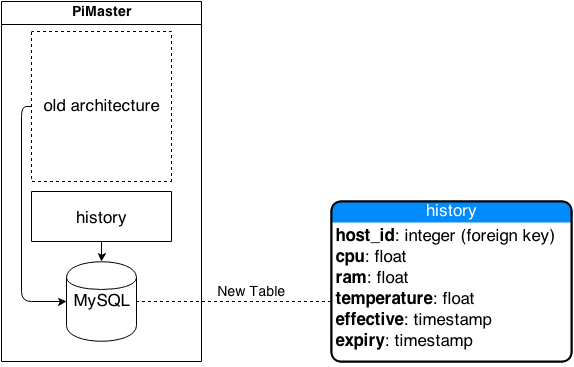
\includegraphics[scale=0.4]{newArch}}
	\caption{Proposed new architecture to allow for history graphs}
	\label{fig:newArch}
\end{figure}

Other functionality in the requirements but not fulfilled at this time are the priority of future work, as well as the changes recommended as a result of the evaluation, outlined in chapter \ref{sec:evaluation}.

The database does not necessarily have to be a MySQL database, and if someone were to want to use, for example, PostgreSQL instead, then this switch should be made easier by making it part of the configuration files.
It may require a different database creation script than the one currently in use but it should be a simple matter of parameterising the database object creation line in the database layer, and using the creation script related to the database the user wants.